\begin{definice}
Nechť $a_k \in \mathbb{R}$ pro $k \in \mathbb{N}_0$ a $b_k \in \mathbb{R}$ pro $k \in \mathbb{N}$. Řadu $\frac{a_0}{2} + \sum_{k=1}^{\infty} \left( a_k \cos (kx) + b_k \sin (kx) \right)$ pro $x \in \mathbb{R}$ nazveme \emph{trigoniometrickou řadou}. Pro dané $n$ je $\frac{a_0}{2} + \sum_{k=1}^{n} \left( a_k \cos (kx) + b_k \sin (kx) \right)$   \emph{trigoniometrický polynom stupně $n$}. $\mathcal{P}_{2 \pi}$ značí množinu všech $2 \pi$-periodických funkcí majících Reimannův integrál na $[0, 2 \pi]$
\end{definice}

Cílem je danou $f \in \mathcal{P}_{2 \pi}$ rozvinout do trigoniometrické řady a:
\begin{enumerate}
\item spočítat $a_k$, $b_k$
\item zjistit, zda-li je řada rovna původní funkci
\end{enumerate}

\begin{vetabd}
Nechť $\{ a_n \}_{n \in \mathbb{N}}$ je posloupnost reálných čísel a $\{ b_n \}_{n=1}^{\infty}$ je nerostoucí posloupnost reálných čísel. Jestliže buď
\begin{enumerate}
\item[(A)] $\sum_{n=1}^{\infty} a_n$ je konvergentní, nebo
\item[(D)] $\lim_{n \rightarrow \infty} b_n = 0$ a $\sum_{n=1}^{\infty} a_n$ má omezené částečné součty
\end{enumerate}
Pak $\sum_{n=1}^{\infty} a_n b_n$ konverguje.
\end{vetabd}

\begin{priklad}
Vyšetřete konvergenci řady
$$\sum_{n=1}^\infty \frac{\sin (nx)}{n}$$
\end{priklad}

\begin{proof}[Řešení]
Pokud $x= \pi k$, $k \in \mathbb{Z} \Leftrightarrow \sum 0 \leftarrow$ konverguje.

Dále předpokládejme, že $x \neq \pi k$. Označme $a_n = \sin (nx)$, $b_n = \frac{1}{n}$. $b_n$ je monotonní nerostoucí a $\lim_{n \rightarrow \infty} b_n = 0$. Nechť $m \in \mathbb{N}$.

$$\left | \sum_{n=a}^{m} \sin (nx) \right | = \left | Im \left( \sum_{n=0}^{m} e^{inx} \right ) \right | = \left | Im \left( \frac{1- \left( e^{ix} \right)^{n+1}  }{1-e^{ix}} \right) \right | \leq \frac{3}{ \left | 1-e^{ix} \right | }$$

Dle Dirichletova kriteria tato suma konverguje.

\end{proof}

\begin{vetal}[o ortogonalitě trigoniometrických funkcí]
\label{o ortogonalitě trigoniometrických funkcí}
Nechť $m, n \in \mathbb{N}$, pak
\begin{eqnarray*}
\int_{0}^{2 \pi} \sin (nx) \cos (mx) dx & = & 0 \\
\int_{0}^{2 \pi} \sin (nx) \sin (mx) dx & = & \pi \textrm{ (pro $n=m$)}, 0 \textrm{ (pro $n \neq m$) } \\
\int_{0}^{2 \pi} \cos (nx) \cos (mx) dx & = & \pi \textrm{ (pro $n \neq m$)}, 0 \textrm{ (pro $n=m$)} 
\end{eqnarray*}
\end{vetal}

\emph{Poznámka} proč se věta jmenuje o ortogonalitě trigoniometrických funkcí? Vraťme se zpět k lineární algebře. Skalární součin vektorů $x$ a $y$ jsme definovali jako $\left\langle x,y \right\rangle = \sum_{i=0}^{n} x_i y_i$. Zcela ekvivalentně byl zaveden skalární součit funkcí $f$ a $g$ jako $\left\langle f, g \right\rangle = \int f(x) g(x) dx$. O vektorech řekneme, že jsou na sebe kolmé (ortogonální), pokud je jejich skalární součin roven nule. Nejinak je tomu i u skalárního součinu funkcí. 

\emph{Poznámka 2} Skalární součin funkcí se nazývá Hilbertovy prostory

\begin{proof}

\begin{eqnarray*}
\sin \alpha \sin \beta & = & \frac{1}{2} \left( \cos (\alpha - \beta) - \cos (\alpha + \beta) \right) \\
\cos \alpha \cos \beta & = & \frac{1}{2} \left( \cos (\alpha - \beta) + \cos (\alpha + \beta) \right) \\
\sin \alpha \cos \beta & = & \frac{1}{2} \left( \cos (\alpha - \beta) + \sin (\alpha + \beta) \right) 
\end{eqnarray*}
Navíc
$$\int \sin(ax) dx = -\frac{\cos (ax)}{a} \textrm { a } \int \cos (ax) dx = \frac{\sin (ax)}{a}$$

$$\int_{0}^{2 \pi} \sin (nx) \cos(mx) = \int_{0}^{2 \pi} \left[ \frac{1}{2} \cos \left( (n-m)x \right) - \frac{1}{2} \left( (n+m)x \right) \right] = $$
Pro $n \neq m$
$$= \left[ \frac{1}{2} \frac{\sin \left( (n-m)x \right)}{n-m} \right]_{0}^{2 \pi} - \left[ \frac{1}{2} \frac{\sin \left( (n+m)x \right)}{n+m} \right]_{0}^{2 \pi} = 0$$
Pro $n=m$
$$=\int_{0}^{2 \pi} \frac{1}{2} \cos 0 + \textrm{(2. člen stejně)} = \pi$$

Zbylé rovnosti analogicky.
\end{proof}\begin{opakovani}[Vlastnosti Reimanovsky integrovantelných funkcí] \quad
\begin{enumerate}
\item $f \in R((a,b)) \Leftrightarrow \forall \varepsilon > 0 \textrm{ dělení } (a,b)$ : $S(f,D) -s(f,D) < \varepsilon$
\item $f \in R((a,b))$ a $f \in R((b,c)) \Leftrightarrow f \in R((a,c))$ pro $a<b<c$
\item $f$ je spojitá na $[a,b] \Rightarrow f \in R((a,b))$
\item $f$ je spojitá na $(a,b)$ a omezená na $[a,b] \Rightarrow f \in R((a,b))$
\item $f, g \in R((a,b)) \Rightarrow f \pm g, f * g \in R((a,b))$
\end{enumerate}
\end{opakovani}

\begin{vetal}[Fourierovy vzorce]
Nechť $f \in \mathcal{P}_{2 \pi}$ a nechť $f(x) = \frac{a_0}{2} + \sum_{k=1}^{\infty} a_k \cos(kx) + b_k \sin(kx)$, nechť navíc řada napravo konverguje stejnoměrně. Pak
\begin{eqnarray*}
a_k & = & \frac{1}{\pi} \int_0^{2 \pi} f(x) \cos(kx) dx, \quad k \in \{0, 1, 2, \ldots\} \\
b_k & = & \frac{1}{\pi} \int_0^{2 \pi} f(x) \sin(kx) dx, \quad k \in \{1, 2, \ldots\} 
\end{eqnarray*}
\end{vetal}

\begin{proof}
Idea důkazu je, že identitu pro $f(x)$ přenásobíme $\cos(kx)$ resp. $\sin(kx)$  a přeintegrujeme přes $[0, 2 \pi]$ a díky Věta L\ref{o ortogonalitě trigoniometrických funkcí} mnoho členů vypadne.

\begin{opakovani}
$f_n \con f$ na $(a,b) \Rightarrow \int_a^b f_n \rightarrow \int_a^b f$
\end{opakovani}

\begin{pozorovani}
$\sum_{k=1}^{\infty} \left( a_k \cos(kx) \sin(lx) + b_k \sin(kx) \sin(lx) \right)$ konverguje stejnoměrně.
\end{pozorovani}

\begin{eqnarray*}
\int_{0}^{2 \pi} f(x) \sin(lx) dx & = & \int_{0}^{2 \pi} \left[ \frac{a_0}{2} \sin(lx) + \sum \left( a_k \cos(kx) \sin(lx) + b_k \sin(kx) \sin(lx) \right) \right] dx \\
& = & b_k \int_{0}^{2 \pi} \sin^2(lx) dx \overset{\textrm{Věta L\ref{o ortogonalitě trigoniometrických funkcí}}}{=} \pi b_k \Rightarrow b_k = \frac{1}{\pi} \int_0^{2 \pi} f(x) \sin(lx) dx
\end{eqnarray*}

podobně přenásobím funkcí $\sin(lx)$ dostanu vzorec pro $a_k$ pro $k \in \mathbb{N}$.

Přenásobím funkcí $\cos(0x) = 1$:

$$\int_{0}^{2 \pi} 1 \cdot f(x) dx = \int_{0}^{2 \pi} \frac{a_0}{2}+0+0+\ldots+0 \Rightarrow a_0 = \frac{1}{\pi} \int_{0}^{2 \pi} f(x) dx = \frac{1}{\pi} \int_0^{2 \pi} f(x) \cos(0x) dx$$

\end{proof}

\begin{definice}
Nehchť $f \in \mathcal{P}_{2 \pi}$. Pak definujeme čísla
\begin{eqnarray*}
a_k & = & \frac{1}{\pi} \int_{0}^{2 \pi} f(x) \cos(kx) dx, \quad k=0,1,\ldots \\
b_k & = & \frac{1}{\pi} \int_{0}^{2 \pi} f(x) \sin(kx) dx, \quad k=1,2,\ldots 
\end{eqnarray*}

a nazveme je \emph{Fourierovými koeficienty} funkce $f$ a 
$$F_f = \frac{a_0}{2} + \sum_{k=1}^\infty a_k \cos(kx) + b_k \sin(kx)$$
nazveme Fourierovou řadou funkce $f$.
\end{definice}

\begin{poznamka}
\begin{itemize} \quad
\item díky $2 \pi$-periodicitě lze funkci integrovat přes libovolný interval délky $2 \pi$ (velmi často $\int_{-\pi}^{\pi}$)
\item Fourierovy řady lze zavést i pro funkce s periodou $l$, pak mají vzorce tvar
\begin{eqnarray*}
F_f & = & \frac{a_0}{2} + \sum_{k=1}^{\infty} a_k \cos \left( \frac{2 k \pi}{l} x \right) + b_k \sin \left( \frac{2 k \pi}{l} x \right) \\
a_k & = & \frac{2}{l} \int_0^{l} f(x) \cos \left( \frac{2 k \pi}{l} x \right) dx \\
b_k & = & \frac{2}{l} \int_0^l f(x) \sin \left( \frac{2 k \pi}{l} x \right) dx 
\end{eqnarray*}
\item někdy se pracuje s rozvoji vůči jinému systému než je trn trigoniometrický
\item je-li $f$ lichá, pak platí $\forall k : a_k = 0$
\item je-li $f$ sudá, pak platí $\forall k : b_k = 0$
\item opecně neplatí $F_f = f$
\end{itemize}
\end{poznamka}

\begin{priklad}
Rozviňte funkci $f(x) = x^2$ do Fourierovy řady na $(-\pi, \pi)$.
\end{priklad}

Funkce $f$ je sudá $\Rightarrow \forall k b_k = 0$.

\begin{eqnarray*}
a_0 & = & \frac{1}{\pi} \int_{-\pi}^{\pi} f(x) dx = \frac{2}{\pi} \int_0^{\pi} x^2 dx = \frac{2}{\pi} \left[ \frac{x^3}{3} \right]_0^\pi = \frac{2}{3} \pi^2 \\
a_k & = & \frac{2}{\pi} \int_{0}^{\pi} x^2 \cos (kx) dx = \frac{2}{\pi} \left( \left[x^2 \frac{\sin (kx)}{k} \right]_0^\pi - \int_0^\pi 2x \frac{\sin (kx)}{k} dx \right) \\
& = & \frac{2}{\pi} \left( 0 - 0 - \frac{2}{k} \int_0^\pi x \sin (kx) dx \right) = \frac{4}{k^2 \pi} \left( \left[ x \frac{\cos (kx)}{k} \right]_0^\pi - \int_0^\pi 1 * \frac{\cos(kx)}{k} dx \right) \\
& = & \frac{4}{k^2 \pi} \left( \pi \cos (k \pi) - 0 - 0 \right) = \frac{4}{k^2} \cos (k \pi) = \frac{4}{k^2} (-1)^k 
\end{eqnarray*}

$$F_f(x) = \frac{1}{3} \pi^2 + \sum_{k=1}^{\infty} \frac{4}{k^2} (-1)^k \cos (kx)$$

\begin{definice}
Nechť $n \in \mathbb{N}$. Pak \emph{Dirichletovým jádrem} nazveme funkci
$$D_n(x) = \frac{1}{2}+\cos(x)+\cos(2x)+\ldots+\cos(nx)$$
\end{definice}

\begin{vetal}[vlastnosti Dirichletova jádra]
Pro Dirichletovo jádro $D_n$ platí
\begin{enumerate}
\item $D_n$ je spojitá, sudá, $2 \pi$-periodická funkce
\item $\int_{-\infty}^{\infty} D_n (x) dx = \pi$
\item $D_n(x) = \frac{\sin \left( n + \frac{1}{2} \right) x}{2 \sin \left( \frac{x}{2} \right)}$, $\forall x \in \mathbb{R} \backslash \bigcup_{k \in \mathbb{Z}} \{ 2k \pi \}$
\end{enumerate}
\end{vetal}

\begin{proof}
\begin{enumerate}
\item plyne bezprostředně z definice
\item $$\int_{-\pi}^\pi \cos(kx) dx = \left[ \frac{\sin(kx)}{k} \right]_{-\pi}^\pi = 0$$
\item
\begin{eqnarray*}
D_n(x) & = & \frac{1}{2} + Re \left( e^{ix} + e^{2ix} + \ldots + e^{nix} \right) = \frac{1}{2} + Re \left( e^{ix} \frac{1-e^{inx}}{1-e^{ix}} \right) \\
& = & \frac{1}{2} + Re \left( \frac{e^{ix} \left( 1-e^{inx} \right) \left( 1-e^{-ix} \right)}{\left( 1-e^{ix} \right) \left( 1-e^{-ix} \right)} \right) \\
& = & \frac{1}{2} + Re \left( \frac{e^{ix} \left( 1-e{-ix}-e{inx}+e{i(n-1)x} \right)}{2-e^{ix}-e^{-ix}} \right) \\
& = & \frac{1}{2} + Re \left( \frac{e^{ix} - 1 - e^{i(n+1)x} + e^{inx}}{2 - 2 \cos(x)} \right) \\
& = & \frac{1}{2} + \frac{\cos(x)-1-\cos(n+1)x + \cos(x)}{2-2\cos(x)} \\
& = & \frac{\cos(mx) - \cos(n+1)x}{2 - 2\cos(x)} \\
& & \textrm{ až sem by to mělo být správně} \\
& = & \frac{-2 \sin \left( n + \frac{1}{2} \right) x \sin \frac{x}{2}}{4 \left( \sin \frac{x}{2} \right)^{2}} = \frac{\sin \left(n + \frac{1}{2} \right) x}{2 \sin \frac{x}{2}} 
\end{eqnarray*}
\end{enumerate}

Pozn.: Důkaz třetí rovnosti je až na znaménko, na přednášce nevyšel. Snad se má použít jiný součtový vzorec goniometrických funkcí (?). Pokud někdo víte, jak to má vyjít, dejte mi prosím vědět.
\end{proof}

\begin{vetal}[částečné součty Fourierovy řady]
Nechť $f \in \mathcal{P}_{2 \pi}$ a $F_f$ je Fourierova řada pro $f$. Potom pro částečné součty $s_n(x) = \frac{a_0}{2} + \sum_{k=1}^{n} (a_k \cos ( kx) + b_k \sin ( kx ))$ platí
$$s_n(x) = \frac{1}{\pi} \int_{-pi}^\pi f(x+z)D_n(y)dy = \frac{1}{\pi} \int_0^\pi \left( f(x+y) + f(x-y) \right) D_n(y) dy$$
\end{vetal}

\begin{proof}
\begin{eqnarray*}
s_n(x) & = & \frac{a_0}{2} + \sum_{k=1}^{n} \left[ a_k \cos(kx) + b_k \sin(kx) \right] \\
& = & \frac{1}{\pi} \int_{-\pi}^\pi \left( \frac{1}{2} + \sum_{k=1}^n \left( \cos(ky) \sin(kx) + \sin(ky) \cos (kx) \right) f(y) dy \right) \\
& = & \frac{1}{\pi} \int_{-\pi}^\pi \left( \frac{1}{2} \cos(k(y-x))  \right) f(y) dy \\
& = & \frac{1}{\pi} \int_{-pi}^\pi D_n(y-x) f(y) dy \\
& = & \frac{1}{\pi} \int_{-\pi}^\pi D_n(t-x) f(t) dt 
\end{eqnarray*}

substituce za $t-x=y$

\begin{eqnarray*}
& = & \frac{1}{\pi} \int_{-\pi -x}^{\pi-x} f(x+y) dy = \frac{1}{\pi} \int_{-\pi}^\pi D_n(y) f(x+y) dy 
\end{eqnarray*}

Dále platí 
$$\int_{-\pi}^\pi = \int_{-\pi}^0 + \int_{0}^\pi$$

Integrál $\int_{-\pi}^0$ spočteme substitucí $y \rightarrow -y$ (korektně bysme měli použít pomocnou proměnnou).

$D_n(y)$ je sudá funkce, proto $f(x+y) \rightarrow f(x-y)$
\end{proof}

\begin{vetat}[Riemann-Lebesqueovo lemma]
\label{Riemann-Lebesqueovo lemma}
Nechť $[a,b] \subset \mathbb{R}$ a $f \in R([a,b])$. Potom
$$\lim_{t \rightarrow \infty} \int_a^b f(x) \cos(tx) dx = 0 \textrm{ a } \lim_{t \rightarrow \infty} \int_a^b f(x) \sin(tx) dx = 0$$
Speciálně pro Fourierovy koeficienty funkce $f \in \mathcal{P}_{2 \pi}$ platí $a_k \rightarrow 0$ a $b_k \rightarrow 0$.
\end{vetat}

\begin{proof}
Nechť $[c,d] \subset [a,b]$ a $f(x) = \chi_{[c,d]}(x)$.

\begin{equation*}
\chi_{[c,d]}(x) = \left\{ \begin{array}{ll}
 1 & x \in [c,d] \\
 0 & \textrm{jinak}
  \end{array} \right.
\end{equation*}

$$\lim_{t \rightarrow \infty} \int_a^b \chi_{[c,d]}(x) \cos(tx) dx = \lim_{t \rightarrow \infty} \int_c^d \cos(tx)dx = \lim_{t \rightarrow \infty} \left[ \frac{\sin(tx)}{t} \right]_c^d = \lim_{t \rightarrow \infty} \frac{\sin(dt) - \sin(ct)}{t} = 0$$

Tvrzení platí pro $\chi_{[c,d]}(x)$, tedy platí pro $\alpha \chi_{[c,d]}(x) \Rightarrow$ pro pevné dělení $D = a = x_0 < x_1 < \ldots < x_m = b$ a $\alpha_i$ platí tvrzení pro
$$f(x) = \sum_{i=1}^m \alpha_i \chi_{[x_{i-1}, x_i]}(x)$$

Nechť nyní $f \in R([a,b])$ a $\varepsilon > 0$. Pak $\exists \textrm{ dělení } D$, že $0 \leq (R) \int_a^b f(x) dy - s(f,D) < \varepsilon$

Označme $$\alpha_i = \min_{x \in [x_{i-1}, x_i]} f(x) \textrm{ a } g(x) = \sum_{i=1}^m \alpha_i \chi_{[x_{i-1}, x_i]} (x)$$ t. j. $(R) \int_a^b g = s(f,D)$.

Víme $\lim_{t \rightarrow \infty} \int_a^b g(x) \cos(tx) = 0$ tedy $\exists t_0 \ \forall t \geq t_0 \textrm{ : } \left| \int_a^b g(x) \cos(tx) dx \right| < \varepsilon$

Nyní pro $t \geq t_0$
$$\left| \int_a^b f(x) \cos(tx) dx \right| \leq \left| \int_a^b (f(x)-g(x)) \cos(tx) dx \right| + \left| \int_a^b g(x) \cos(tx) dx \right| \leq$$
Poznamenejme $f(x) \geq g(x) \Rightarrow f(x)-g(x) \geq 0 \textrm{ : } \left| \int F(x) \right| \leq \int \left| F(x) \right|$
$$\leq \int_a^b (f(x)-g(x)) |\cos(tx)| dx + \varepsilon \leq \int_a^b f(x) dx - \int_a^b g(x) dx + \varepsilon < 2 \varepsilon$$

Pro sinus budeme postupovat analogicky
\end{proof}

\begin{vetat}[Diniho kriterium]
Nechť $f \int \mathcal{P}_{2 \pi}$ a $x \in \mathbb{R}$. Nechť existují vlastní limity $f(x+) = \lim_{y \rightarrow x+} f(y)$ a $f(x-) = \lim_{y \rightarrow x-} f(y)$ a nechť existují vlastní limity
$$\lim_{y \rightarrow x+} \frac{f(y)-f(x+)}{y-x} \quad \mathrm{a} \quad \lim_{y \rightarrow x-} \frac{f(y)-f(x-)}{y-x}$$
Potom Fourierova řada funkce $f$ konverguje v bodě $x$ k hodnotě $\frac{f(x+) + f(x-)}{2}$.
\end{vetat}

\begin{dusledek}
Nechť $x \in \mathbb{R}$ a nechť pro $f \in \mathcal{P}_{2 \pi}$ existuje $f^\prime (x)$. Potom $f(x)=F_f(x)$.
\end{dusledek}

\begin{priklad}
\begin{itemize}
\item $f(x) = x^2$ pro $x \in [-\pi, \pi)$
\begin{figure}[h]
\begin{center}
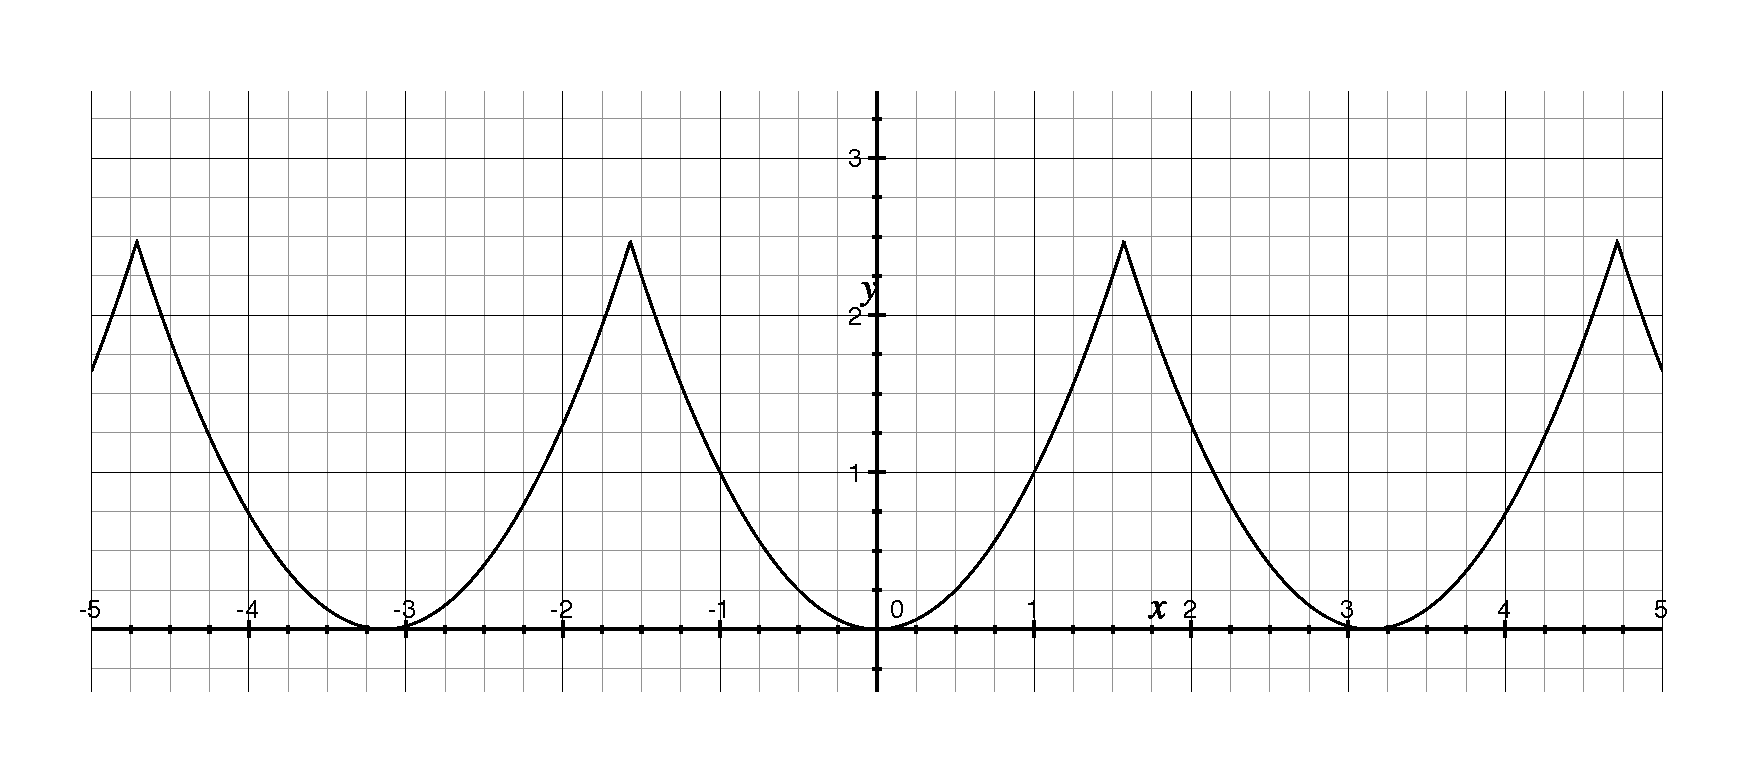
\includegraphics[scale=0.2]{grafy/graf1.eps}
\end{center}
\end{figure}
v bodě $x = \pi$ konverguje k $\pi^2$

\item $f(x) = x^2$ pro $x \in [0,2 \pi)$
\begin{figure}[h]
\begin{center}
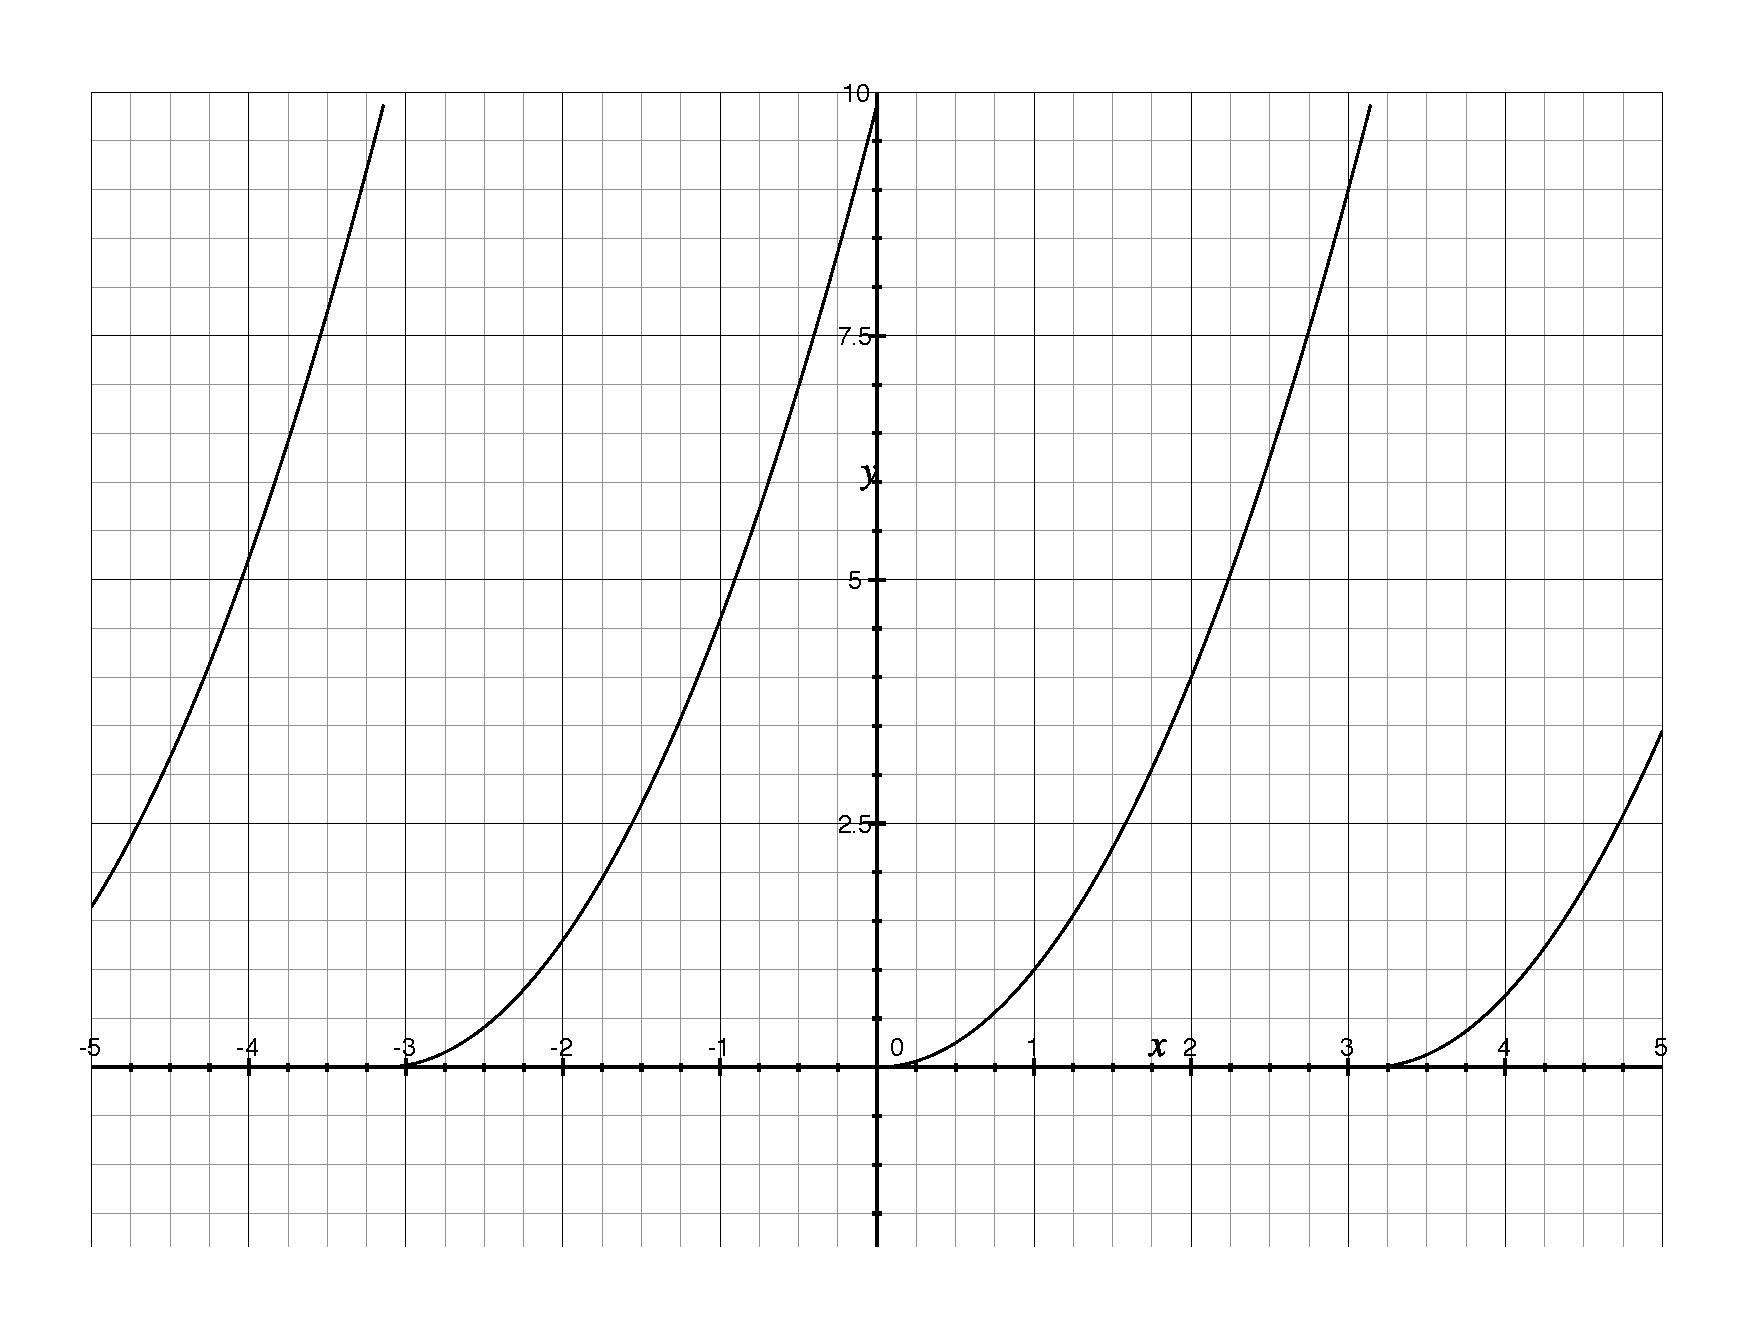
\includegraphics[scale=0.2]{grafy/graf2.eps}
\end{center}
\end{figure}
v bodě $x = 2\pi$ konverguje k $2\pi^2$

\end{itemize}
\end{priklad}


\begin{proof}
Chceme $F_f(x) = \frac{f(x+) + f(x-)}{2}$, tedy $s_n(x) \overset{n \rightarrow \infty}{\rightarrow}$

\begin{eqnarray*}
s_n(x) - \frac{f(x+)+f(x-)}{2} & = & \frac{1}{\pi} \int_0^\pi \left( f(x+y) + f(x-y) \right) D_n(y) dy - \frac{f(x+) + f(x-)}{2} \frac{2}{\pi} \int_0^\pi D_n(y)dy \\
& \overset{V5, VL4 (ii)}{=} & \frac{1}{\pi} \int_0^\pi \left( f(x+y) - f(x+) + f(x-y) - f(x-) \right) D_n(y) dy \\
& \overset{VL4(iii)}{=} & \frac{1}{\pi} \int_{0}^\pi \underbrace{\left( \frac{f(x+y) - f(x+) + f(x-y) - f(x-)}{2 \sin \left( \frac{y}{2} \right)} \right)}_{\textrm{pokud $\in R([0,\pi])$, pak VT\ref{Riemann-Lebesqueovo lemma} dokončí důkaz}} \sin \left( n + \frac{1}{2} \right)y dy 
\end{eqnarray*}

Chceme $F(y) = \frac{f(x+y) - f(x+) + f(x-y) - f(x-)}{2 \sin \left( \frac{y}{2} \right)} \in R([0,\pi])$. 

Existuje
$$\lim_{y \rightarrow 0} F(y) = \lim_{x \rightarrow 0} \frac{y}{2 \sin \left( \frac{x}{2} \right)} \lim_{y \rightarrow 0} \left( \frac{f(x+y)-f(x+)}{y} + \frac{f(x-y)-f(x-)}{y} \right) = A \in \mathbb{R}$$

\begin{tvrzeni}
$h \in R([a,b])$ spojitá na $[a,b]$, $0 < \delta \leq g \leq D$. Pak $\frac{h}{g} \in R([a,b])$.
\end{tvrzeni}

Nechť $\varepsilon > 0 \ \exists \delta > 0 \ \forall y \in [0, \delta] \textrm{ : } |F(y)-A| < \varepsilon$

Nyní $\delta$ je pevné a tedz dle tvrzení $F(y) \in R([\delta, \pi])$, $g(y) = 2 \sin \frac{y}{2}$.

Tedy $\exists \overline{D}$ dělení $[\delta, \pi]$ že $S(F,\overline{D}) - s(f,\overline{D}) < \varepsilon$.

Nechť $D$ je dělení $[0,\pi]$ mající interval k $\overline{D}$ a interval k $[0, \delta]$. Pak 
$$S(F, D)-s(f,D) = \left( \max_{x \in [0, \delta]} F(x) - \min_{x \in [0, \delta]} F(x) \right) \delta + S(F, \overline{D}) - s(F, \overline{D}) \leq 2 \varepsilon \delta + \varepsilon \leq \varepsilon (2 \pi + 1)$$
\end{proof}

\begin{vetabd}[Jordan-Dirichletovo kriterium]
Nechť $f \in \mathcal{P}_{2\pi}$ je po částech monotónní. Tedy nechť existuje konečně mnoho bodů $0=a_1 < a_2 < \ldots < a_m = 2 \pi$ tak, že $f$ je monotónní na $(a_i, a_{i+1})$ pro $i \in \{1, \ldots, m-1 \}$. Potom Fourierova řada funkce $f$ konverguje v bodě $x$ k hodnotě $\frac{f(x+) + f(x-)}{2}$ pro všechna $x \in \mathbb{R}$.
\end{vetabd}